\documentclass{article}
\usepackage{tikz}
\usetikzlibrary{arrows.meta}

\begin{document}

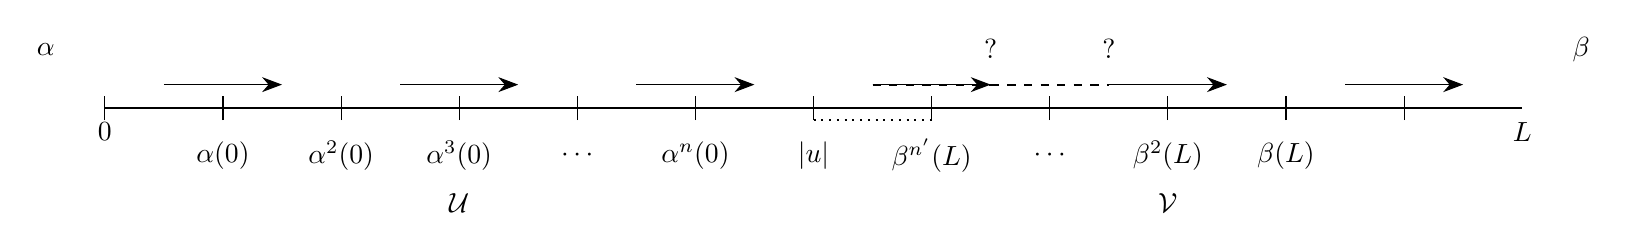
\begin{tikzpicture}[scale=1.5]
    % Draw the horizontal line
    \draw[thick] (0,0) -- (12,0);
    
    % Label the endpoints
    \node at (0,-0.2) {$0$};
    \node at (12,-0.2) {$L$};
    
    % Draw vertical lines
    \foreach \x in {0, 1, ..., 11} {
        \draw (\x, -0.1) -- (\x, 0.1);
    }
    
    % Label the points on the left side
    \node at (1, -0.4) {$\alpha(0)$};
    \node at (2, -0.4) {$\alpha^2(0)$};
    \node at (3, -0.4) {$\alpha^3(0)$};
    \node at (4, -0.4) {$\cdots$};
    \node at (5, -0.4) {$\alpha^n(0)$};
    \node at (6, -0.4) {$|u|$};
    
    % Label the points on the right side
    \node at (7, -0.4) {$\beta^{n'}(L)$};
    \node at (8, -0.4) {$\cdots$};
    \node at (9, -0.4) {$\beta^2(L)$};
    \node at (10, -0.4) {$\beta(L)$};
    
    % Draw the labels for alpha and beta
    \node at (-0.5, 0.5) {$\alpha$};
    \node at (12.5, 0.5) {$\beta$};
    
    % Draw the dashed line
    \draw[dotted, thick] (6, -0.1) -- (7, -0.1);
    
    % Draw the arrows
    \draw[-{Stealth[scale=1.5]}] (0.5, 0.2) -- (1.5, 0.2);
    \draw[-{Stealth[scale=1.5]}] (2.5, 0.2) -- (3.5, 0.2);
    \draw[-{Stealth[scale=1.5]}] (4.5, 0.2) -- (5.5, 0.2);
    \draw[-{Stealth[scale=1.5]}] (6.5, 0.2) -- (7.5, 0.2);
    \draw[-{Stealth[scale=1.5]}] (8.5, 0.2) -- (9.5, 0.2);
    \draw[-{Stealth[scale=1.5]}] (10.5, 0.2) -- (11.5, 0.2);
    
    % Draw the question marks
    \draw[dashed, thick] (6.5, 0.2) -- (7.5, 0.2);
    \draw[dashed, thick] (7.5, 0.2) -- (8.5, 0.2);
    
    \node at (7.5, 0.5) {?};
    \node at (8.5, 0.5) {?};
    
    % Draw the labels u and v
    \node at (3, -0.8) {$\mathcal{U}$};
    \node at (9, -0.8) {$\mathcal{V}$};
\end{tikzpicture}

\end{document}